\section{Stability study}\label{sec:dem-stability}
As mentioned when the integration algorithm was introduced in \cref{sec:particle-dynamics}, the velocity-Verlet algorithm is a computationally efficient, second-order accurate means of updating the kinematics of all the particles in the ensemble\cite{Kruggel-Emden2008}. The timestep of the integration, however, must often be very small to ensure that it is less than the time taken for a pressure wave to propagate through the particle. The timestep is further constrained by the quasistatic assumption used to derive the Hertzian contact force such that inertial and relaxation effects may be neglected\cite{Brilliantov1996}. We will also show that, in order to avoid heat energy to propagate further than a single pebble during a single timestep, the thermal timestep requirement is orders of magnitude larger than the mechanical timestep equivalent. And that the overall minimum timestep is thus driven by the mechanical stability.

In tandem with the requirement on very small timestep, the thermal time-constants in the ceramic breeder zones can be many hundreds of seconds. These two conditions seem to conspire to force an unacceptably large requirement on the number of timesteps for a thermal DEM simulation and thus make numerical experiments impractical.

In this section we will analyze the calculation of a critical timestep based on the speed of a Rayleigh wave propagating along the surface of a particle. Then, with that knowledge in hand, we will argue for scaling certain physical properties to allow for faster simulations without sacrificing fidelity to the real physics of the problem.


%~~~~~~~~~~~~~~~~~~~~~~~~~~~~~~~~~~~~~~~~~~~~~~~~~~~~~~~~~~~~~~~~~~~~~~~~~~~~~~~~
\subsection{Critical dynamic timestep}
If we wish to choose a timestep sufficiently small such that a pressure wave originating from the contact of one particle does not propagate to other neighboring particles during the timestep, we must choose a timestep smaller than the critical timestep defined by Rayleigh wave traveling through the solid.

When a force is applied to the surface of an elastic body, the force propagates along the surface at the wave speed first solved by John William Strutt, 3rd Baron Rayleigh\cite{Rayleigh1885} (when he wasn't discovering the scattering phenomenon explaining why the sky is blue or winning the Nobel prize for discovering Argon),

\begin{equation}
	u_{\Ra} = K\sqrt{\frac{G}{\rho}}
\end{equation}

where, again, $G$ is the shear modulus and $\rho$ is the density of the elastic material. The $K$ coefficient is a complicated function coming from Rayleigh's solution but can be approximated as\cite{Sheng2004}

\begin{equation}
	K = 0.1631 \nu + 0.876605
\end{equation}

which is valid for realistic values of Poisson's ratio, $\nu$, of elastic materials. From the inverse of the Rayleigh wave frequency, we can directly find a timestep for Rayleigh waves on a sphere of radius, $R$,

\begin{equation}\label{eq:rayleigh-stability-time}
	\delta t_{\Ra} = \frac{\pi R}{u_{\Ra}}
\end{equation}

When we write this for any particle, $i$ in the ensemble (exchanging the shear for elastic modulus),

\begin{equation}\label{eq:rayleigh-timestep}
	(\delta t_{\Ra})_i = \frac{\pi R_i }{0.1631 \nu_i + 0.876605} \sqrt{\frac{2(1+\nu_i)\rho_i}{E_i}}
\end{equation}

We allow for the particles in the system to have varying density, elastic modulus, and size. Therefore the critical timestep for the entire system is governed by the minimum value of any particle's Rayleigh timestep. 

\begin{equation}
	\delta t_c = \min_{\forall i}\left[(\delta t_{\Ra})_i\right]
\end{equation}


% \begin{align}
% \delta t_c = \eta  \sqrt{\frac{m_0}{k_0}}
% \end{align}
% where $m_0$ is the smallest particle mass, related to the smallest particle radius, $R_0$. The value of $\eta$ is less than unity and depends on the integration algorithm as well as dimensions of freedom [site O'Sullivan].
% \begin{align}
% m_0 = \frac{4}{3} \pi R_0^3 \rho
% \end{align}
% and we assume all pebbles have the same density, $\rho$. $k_0$ is the maximum normal stiffness in the ensemble. The timestep chosen for the DEM must be less than this critical timestep.
% \begin{align}
% \Delta t \le \delta t_c
% \end{align}

% From Hertz theory, the maximum normal contact stiffness is
% \begin{align}
% k_0 = \frac{4}{3} E^* \sqrt{R^*_0 \delta_0}
% \end{align}

% To find the maximum contact stiffness (neglecting the influence of $\delta_0$ for the moment), we will express the relative radius in an alternate form,
% \begin{align}
% \frac{1}{R^*_0} = \frac{1}{R_0} + \frac{1}{\gamma R_0}
% \end{align}
% where $\gamma \ge 1$, it is a parameter that indicates our smallest pebble of radius $R_0$ is interacting with another pebble that is either the same size or larger. In the limits, if $\gamma =1$, then $R^*_0 = \frac{R_0}{2}$. If $\gamma \rightarrow \infty$, then $R^*_0 = R_0$. The stiffness is positively proportional to relative radius. Therefore if we desire the maximum contact stiffness, we need the largest value of $R^*_0$ and thus require $\gamma \rightarrow \infty$.

% With $R^*_0 = R_0$, we use this in the formula for pebble mass term of the stability criteria 
% \begin{align}
% \delta t_c &= \eta  \sqrt{\frac{\frac{4}{3} \pi (R^*_0)^3 \rho}{\frac{4}{3} E^* \sqrt{R^*_0 \delta_0}}}\\
% \delta t_c &= \left[ \eta \sqrt{ \pi} \right] \rho^{1/2}\left(\frac{1}{E^*}\right)^{1/2} \left(\frac{1}{\delta_0}\right)^{1/4}(R^*_0)^{5/4}
% \end{align}

% We can relate the maximum pebble overlap $\delta_0$ to the maximum contact force in the ensemble with Eq.~\ref{eq:hertzForce}, after some algebra we find
% \begin{align}
% \delta t_c &= \left[ \eta \sqrt{ \pi} (4/3)^{1/6} \right] \rho^{1/2} \left(\frac{1}{F_\text{max}}\right)^{1/6} \left(\frac{1}{E^*}\right)^{1/3} R^{*5/4}_0
% \end{align}

% The term in the bracket is a constant near unity. Neglecting it, we see the timestep is proportional to these terms,
% \begin{align}\label{eq:stability-terms}
% \delta t_c \propto \rho^{1/2} \left(\frac{1}{F_\text{max}}\right)^{1/6} \left(\frac{1}{E^*}\right)^{1/3} R^{*5/4}_0
% \end{align}

% Figure~\ref{fig:stability-curves} provides visual reinforcement of the powers of terms in Eq.~\ref{eq:stability-terms}; it is the impact of different normal-contact parameters on the stable timestep. 
% \begin{figure}[ht!]
% \centering
% 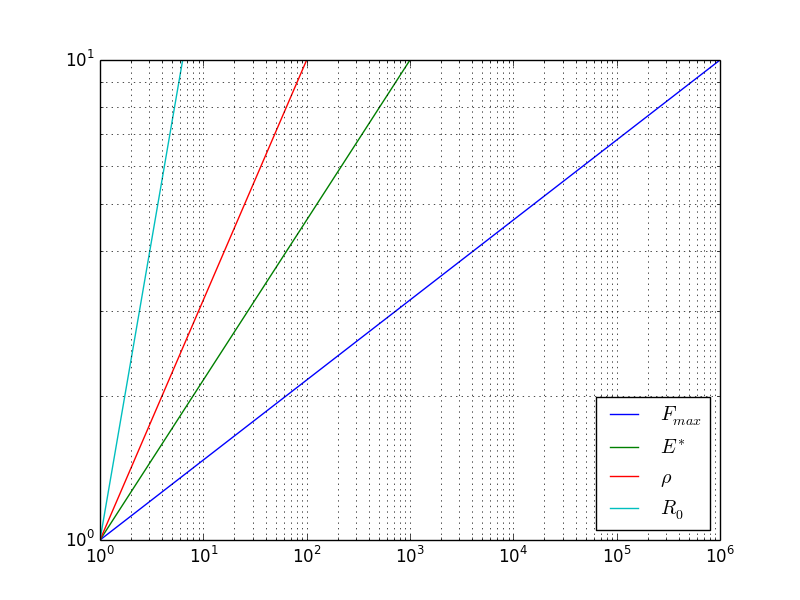
\includegraphics[width = 0.75 \textwidth]{chapters/figures/stability_curves}
% \caption{Curves showing the rate of response to timestep on the various normal-contact parameters.}\label{fig:stability-curves}
% \end{figure}

% It is apparent that simulations become less stable primarily as the pebble diameter decreases and then slightly less so for decreasing density and increasing the effective Young's modulus. It takes a rather large increase in the maximum contact force to cause the stable timestep to decrease. This is a fortunate result as it is primarily material properties which dictate stability of a DEM simulation. If external pressures increase and cause increases in the maximum normal contact force in the ensemble, it is unlikely to cause instabilities in the model. The result also provides insight into scaling of physical parameters to allow larger timesteps and thereby shorter overall duration of simulations.

The ceramic materials identified for breeders have relatively high Young's moduli, on the order of \si{10^{10} Pa}. The smallest radius will be on the order of \si{10^{-4} m}. The ceramic density is approximately on the scale of \si{10^{4} kg/m^3}. These values lead to a necessary timestep of

\begin{equation}
	\delta t_c \propto 10^{-7} \si{s}
\end{equation}

For a simulation that may last several hundreds of seconds of real time, this then requires more than 10$^9$ timesteps. If we have 10$^4$ particles in the simulation, each having their position integrated over a billion times, it becomes obvious that computational time is a major issue for our simulations of nuclear heating of ceramic breeder pebbles. If we are able to reduce the critical timestep (while perhaps decreasing the simulation time), the simulations will be much more practical for research use.
%~~~~~~~~~~~~~~~~~~~~~~~~~~~~~~~~~~~~~~~~~~~~~~~~~~~~~~~~~~~~~~~~~~~~~~~~~~~~~~~~




%~~~~~~~~~~~~~~~~~~~~~~~~~~~~~~~~~~~~~~~~~~~~~~~~~~~~~~~~~~~~~~~~~~~~~~~~~~~~~~~~
\subsection{Critical thermal timestep}

In \cref{sec:ht-pebble-conduction}, we introduced the dynamics of heat transfer between contacting particles in an ensemble. As we integrate the energy of an individual particle in time, we must also ensure that energy would not propagate through a particle faster than a single timestep can capture. In analogy to the critical timestep for mechanical stability (e.g. Eq.\ref{eq:rayleigh-stability-time}), we write for particle $i$,

\begin{equation}
	\delta t_\Bi = \frac{\rho_i C_i V_i}{H_c}
\end{equation}

where $\rho_i C_i V_i$ represents the inertial resistance to changing the temperature of $T_i$ and the conductance, $H_c$ represents the speed at which energy is delivered to $T_i$ from contact conduction. Then from the definition of $H_c$ we have given for smooth elastic spheres, this is also written as

\begin{equation}
	\delta t_\Bi = \frac{(4/3)\pi R_i^2\rho_i C_i}{2k^*}\frac{R_i}{a}
\end{equation}

For the material properties of lithium ceramics, as discussed for mechanical stability, we can expect

\begin{equation*}
	\frac{(4/3)\pi R_i^2\rho_i C_i}{2k^*} \approx \frac{(10^{-4})^210^{4}10^3}{10^0} = 10^{-1}
\end{equation*}

But from the requirements on Hertz theory in \cref{sec:hertz-contact}, we have required that $\frac{a}{R_i} \ll 1$. Thus the timestep for stability in the energy calculation is utterly negligible compared to the mechanical stability.

Vargas and McCarthy\cite{Vargas2001} make similar arguments, giving the criteria as,

\begin{equation}
	\frac{\mathrm{d}T_i}{T_i - T_j} \ll 1
\end{equation}

and too note that the timestep requirement for thermal calculations are orders of magnitude less restrictive than the analogous restriction of the particle dynamics.

Thus we can be confident that any timestep chosen for dynamic stability in the DEM simulation will automatically satisfy the timestep for thermal stability. 
%~~~~~~~~~~~~~~~~~~~~~~~~~~~~~~~~~~~~~~~~~~~~~~~~~~~~~~~~~~~~~~~~~~~~~~~~~~~~~~~~





%~~~~~~~~~~~~~~~~~~~~~~~~~~~~~~~~~~~~~~~~~~~~~~~~~~~~~~~~~~~~~~~~~~~~~~~~~~~~~~~~
\subsection{Simulation acceleration with scaled material properties}

We rewrite Eq.~\ref{eq:rayleigh-timestep} to facilitate a discussion on the parameters. Isolating each material term (neglecting the Poisson ratio) gives, 

\begin{equation}
	\delta t_c \propto R_i \times \rho_i^{1/2} \times E_i^{-1/2}
\end{equation}

% [pretty sure the approximation for $\nu$ only works when it's less than 1 so can't scale. must find out for sure.]

% The most direct effect would come from scaling the radius 





% From Makse\cite{Makse2004}

% We choose the time step to be a fraction of the time that it takes for a sound wave to propagate on the grain. Moreover, the quasistatic approximation used to calculate the Hertz force is valid only when the relative velocities of the par- ticles is smaller than the speed of sound in the grains\cite{Brilliantov1996}. Thus the characteristic time is $t_0 = R\sqrt{\rho_r/\mu_r}$ Typically, one chooses a time interval much smaller than the characteristic time, then $\Delta t=aR \sqrt{\rho_r/\mu_r}$ with $a<1$. Typical values for glass beads are:
% \si{\rho =2600 kg/m^3}, \si{\mu_r = 29 GPa}, \si{R = 0.1 mm}. Then $\Delta t$ should be smaller than \si{10^{−8} s}. Thus in order to perform a simulation over one second, more than $10^8$ steps are needed, which is obviously a very intensive computation. In this case, it is customary to increase the density or decrease the rigidity of the particles to allow for a larger time step to integrate the equations of motion over realistic periods of time. If the shear modulus of the grains in decreased, then it should be checked that the resulting stresses are several order of magnitude smaller than $\mu_r$, thus ensuring the condition of a nearly rigid system even though $\mu_r$ is taken smaller to obtain larger timesteps.